\documentclass[12pt]{article}
\usepackage{amsmath}
\usepackage[english]{babel}
\usepackage{graphicx}
\usepackage{verbatim}
\usepackage{wrapfig}
\usepackage{float}
\usepackage[top=1in, bottom=1in, left=1in, right=1in]{geometry}
\usepackage{times}
\usepackage{hyperref}
\hyphenpenalty=5000
\tolerance=1000
\setlength\parindent{0pt}
\begin{document}
\title{Network Simulation}
\author{Maxwell Horton, Alex Jose, Michael Lauria, Anish Agarwal, Johno Ikpeazu}


\maketitle
\noindent
\tableofcontents
\newpage
\section{Introduction}

\begin{figure}[t]
\centering 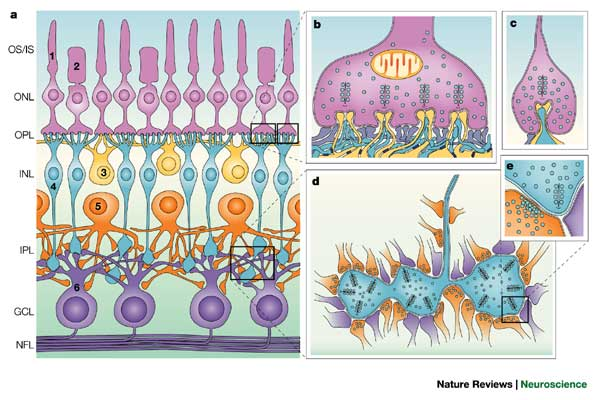
\includegraphics[scale=1.]{figures/cells_2.jpg}
\caption{Examples of cells of the retina. Taken from \cite{wassle}.}
\label{fig:test}
\end{figure}

\section{Code}
\section{Analysis}
\subsection{Test Case 0}
\subsection{Test Case 1}
\subsection{Test Case 2}
\section{Difficulties}

\end{document}
